\section{Experiments}
This section focuses on the results gotten from the conducted experiments. These will first briefly be presented in section \ref{results}. After that, section \ref{exp:int} will discuss them in more detail, and see how they compare to earlier studies, etc.

\subsection{Results} \label{results}
Results are presented in the form of tables and line plots. The former of these report final testing performance, whereas the latter mostly visualise validation accuracy during training.

To give a more precise description: tables show average testing performance over the 5 trials per experiment, with standard deviation ($s$) as subscript. Besides accuracy, also balanced accuracy is reported. This measure is defined as the average recall over all classes, such that it penalises errors on less occurring classes more than plain accuracy would. Lastly, green shaded cells mark best performance, while yellow and red mark second best and worst performance, respectively.

For line plots, shaded regions correspond to the \textit{standard error of the mean} ($\pm s \div \sqrt{N}$, where $N=5$). In cases where they show average validation accuracy, plots end when an early stop occurred for the first of 5 trials. To easily distinguish VTs from CNNs, VTs are plotted with continues lines, and CNNs with dashed ones.

\subsubsection{Off the shelf learning} \label{results:ots}

\begin{figure*}[tb]
    \centering
    \def\svgwidth{\textwidth}
    \input{img/ots_mean_accuracy.pdf_tex}
    \caption{Average validation accuracy when training with an off the shelf learning scheme. It can be observed that the \texttt{Swin} VT achieves the highest performance overall, but with the \texttt{ConvNext} CNN being a close second. More general, VTs perform on par with CNNs, if not slightly better.}
    \label{results:img:ots}
\end{figure*}

\begin{table*}[tb]
\centering
\resizebox{\textwidth}{!}{%
\begin{tabular}{lllllll}
\hline
\textbf{Model} & \textbf{Type} &  & \textbf{Material} & & \textbf{Artist} & \\
& \textbf{Accuracy} & \textbf{Bal. accuracy} & \textbf{Accuracy} & \textbf{Bal. accuracy} & \textbf{Accuracy} & \textbf{Bal. accuracy} \\ \hline
\textbf{vit\_b\_16} & 86.06\% $_{\pm 1.06\%}$ & 84.13\% $_{\pm 1.57\%}$ & 81.78\% $_{\pm 0.48\%}$ & 67.38\% $_{\pm 1.37\%}$ & 84.89\% $_{\pm 0.46\%}$ & 81.42\% $_{\pm 0.42\%}$  \\
\textbf{swin\_b} & \cellcolor{bestcol}89.43\% $_{\pm 0.93\%}$ & \cellcolor{bestcol}87.47\% $_{\pm 1.02\%}$ & \cellcolor{bestcol}85.87\% $_{\pm 0.35\%}$ & \cellcolor{bestcol}71.19\% $_{\pm 1.60\%}$ & \cellcolor{bestcol}90.40\% $_{\pm 0.65\%}$ & \cellcolor{bestcol}88.64\% $_{\pm 0.78\%}$  \\
\textbf{beit\_b\_16} & \cellcolor{worstcol}82.26\% $_{\pm 0.72\%}$ & \cellcolor{worstcol}77.75\% $_{\pm 0.27\%}$ & 76.87\% $_{\pm 0.96\%}$ & 60.16\% $_{\pm 1.56\%}$ & 79.70\% $_{\pm 0.69\%}$ & 75.35\% $_{\pm 1.09\%}$  \\
\textbf{deit\_b\_16} & 88.18\% $_{\pm 0.66\%}$ & 85.36\% $_{\pm 0.54\%}$ & 82.80\% $_{\pm 1.12\%}$ & 66.46\% $_{\pm 1.03\%}$ & 88.13\% $_{\pm 0.76\%}$ & 85.62\% $_{\pm 0.87\%}$  \\\hdashline
\textbf{vgg19} & 83.93\% $_{\pm 0.72\%}$ & 83.35\% $_{\pm 0.81\%}$ & 76.87\% $_{\pm 0.44\%}$ & 61.39\% $_{\pm 1.47\%}$ & 82.01\% $_{\pm 0.66\%}$ & 78.10\% $_{\pm 0.77\%}$  \\
\textbf{resnet50} & 85.51\% $_{\pm 0.64\%}$ & 82.33\% $_{\pm 1.85\%}$ & 80.99\% $_{\pm 0.82\%}$ & 65.51\% $_{\pm 0.93\%}$ & 87.71\% $_{\pm 1.06\%}$ & 85.12\% $_{\pm 1.34\%}$  \\
\textbf{eff. netv2\_m} & 83.41\% $_{\pm 0.76\%}$ & 82.05\% $_{\pm 1.25\%}$  & \cellcolor{worstcol}75.96\% $_{\pm 1.24\%}$ & \cellcolor{worstcol}59.15\% $_{\pm 1.24\%}$ & \cellcolor{worstcol}78.62\% $_{\pm 1.07\%}$ & \cellcolor{worstcol}73.92\% $_{\pm 0.96\%}$  \\
\textbf{convnext\_b} & \cellcolor{secondbestcol}89.19\% $_{\pm 0.64\%}$ & \cellcolor{secondbestcol}86.95\% $_{\pm 1.38\%}$ & \cellcolor{secondbestcol}84.14\% $_{\pm 0.92\%}$ & \cellcolor{secondbestcol}69.10\% $_{\pm 1.05\%}$ & \cellcolor{secondbestcol}90.13\% $_{\pm 0.94\%}$ & \cellcolor{secondbestcol}87.84\% $_{\pm 1.07\%}$  \\\hline
\end{tabular}
}
\caption{Testing performance after off the shelf learning. Results are similar to validation accuracy shown in figure \ref{results:img:ots}, with \texttt{Swin} and \texttt{ConvNext} showing respective best and second best performance in all cases.}
\label{results:tab:ots}
\end{table*}

Table \ref{results:tab:ots} shows testing performance of OTS trained models on the 3 classification tasks, while figure \ref{results:img:ots} shows corresponding validation accuracies. Performance on the testing set is comparable among all tasks in terms of rankings. Other observations are consistent as well, such as \texttt{ConvNext} taking the most epochs to converge.

VTs perform very much on par with CNNs, if not slightly better. The best performing model, for instance, is the \texttt{Swin} VT, which shows the highest testing performance without exception. Moreover, all VTs except \texttt{BeiT} are positioned relatively high in the rankings. This is also reflected in their combined average accuracies being higher than those of CNNs. To give \textit{Type classification} as an example: here VTs as a group achieve an 86.5\% mean accuracy, while this is 85.5\% for CNNs.

Finally, when comparing the 3 classification tasks to one another, it can be observed that highest overall accuracies are achieved for \textit{Artist classification}, and lowest ones for \textit{Material classification}. For balanced accuracy the differences are more extreme, as this measure also falls behind plain accuracy the most for \textit{Material classification}, and the least for \textit{Artist classification}.

% Results favorable for VTs:
%    - Best performing model = VT (SWIN)
%    - 3 of 4 VTs on top ?
%    - Avg of all VTs better than avg CNNs

% Talk about differences between experiments
% Talk about balanced accuracy?

\subsubsection{Fine-tuning} \label{results:ft}

\begin{figure*}[tb]
    \centering
    \def\svgwidth{\textwidth}
    \input{img/ft_mean_accuracy.pdf_tex}
    \caption{Average validation accuracy when fine-tuning models on the target task. Overall, performance is higher compared to off the shelf learning in figure \ref{results:img:ots}, while the differences between models are also smaller here. The \texttt{Swin} VT and \texttt{ConvNext} CNN remain the best performing models, while in general, results are less favourable for VTs than they were for off the shelf learning.}
    \label{results:img:ft}
\end{figure*}

\begin{table*}[tb]
\centering
\resizebox{\textwidth}{!}{%
\begin{tabular}{lllllll}
\hline
\textbf{Model} & \textbf{Type} &  & \textbf{Material} & & \textbf{Artist} & \\
& \textbf{Accuracy} & \textbf{Bal. accuracy} & \textbf{Accuracy} & \textbf{Bal. accuracy} & \textbf{Accuracy} & \textbf{Bal. accuracy} \\ \hline
\textbf{vit\_b\_16} & \cellcolor{worstcol}90.11\% $_{\pm 0.35\%}$ & 87.40\% $_{\pm 0.29\%}$ & 87.42\% $_{\pm 0.45\%}$ & 73.46\% $_{\pm 1.44\%}$ & 92.05\% $_{\pm 0.44\%}$ & 89.77\% $_{\pm 0.38\%}$  \\
\textbf{swin\_b} & \cellcolor{bestcol}92.17\% $_{\pm 0.98\%}$ & \cellcolor{secondbestcol}89.71\% $_{\pm 1.03\%}$ & \cellcolor{bestcol}89.35\% $_{\pm 0.68\%}$ & 77.16\% $_{\pm 2.98\%}$ & \cellcolor{bestcol}95.05\% $_{\pm 0.47\%}$ & \cellcolor{bestcol}93.94\% $_{\pm 0.81\%}$  \\
\textbf{beit\_b\_16} & 90.81\% $_{\pm 0.41\%}$ & 87.95\% $_{\pm 0.69\%}$ & \cellcolor{worstcol}85.74\% $_{\pm 0.37\%}$ & \cellcolor{worstcol}72.12\% $_{\pm 1.38\%}$ & \cellcolor{worstcol}91.27\% $_{\pm 1.13\%}$ & \cellcolor{worstcol}88.83\% $_{\pm 1.63\%}$  \\
\textbf{deit\_b\_16} & 91.78\% $_{\pm 0.64\%}$ & 89.22\% $_{\pm 0.90\%}$ & 87.85\% $_{\pm 1.12\%}$ & 74.42\% $_{\pm 1.99\%}$ & 93.37\% $_{\pm 1.15\%}$ & 91.67\% $_{\pm 1.55\%}$  \\\hdashline
\textbf{vgg19} & 90.54\% $_{\pm 0.37\%}$ & \cellcolor{worstcol}87.05\% $_{\pm 1.03\%}$ & 85.74\% $_{\pm 1.40\%}$ & 72.43\% $_{\pm 3.03\%}$ & 92.20\% $_{\pm 0.49\%}$ & 90.18\% $_{\pm 0.72\%}$  \\
\textbf{resnet50} & 91.78\% $_{\pm 0.44\%}$ & 88.24\% $_{\pm 0.59\%}$ & 88.69\% $_{\pm 0.99\%}$ & \cellcolor{secondbestcol}77.97\% $_{\pm 2.25\%}$ & \cellcolor{secondbestcol}94.72\% $_{\pm 0.74\%}$ & \cellcolor{secondbestcol}93.41\% $_{\pm 1.05\%}$  \\
\textbf{eff. netv2\_m} & 90.87\% $_{\pm 0.67\%}$ & 88.34\% $_{\pm 1.37\%}$ & 87.55\% $_{\pm 1.15\%}$ & 75.31\% $_{\pm 1.60\%}$ & 92.65\% $_{\pm 0.54\%}$ & 90.84\% $_{\pm 0.51\%}$  \\
\textbf{convnext\_b} & \cellcolor{secondbestcol}92.15\% $_{\pm 0.40\%}$ & \cellcolor{bestcol}89.82\% $_{\pm 1.18\%}$ & \cellcolor{secondbestcol}88.79\% $_{\pm 1.07\%}$ & \cellcolor{bestcol}78.40\% $_{\pm 1.26\%}$ & 94.60\% $_{\pm 0.54\%}$ & 93.13\% $_{\pm 0.61\%}$  \\\hline
\end{tabular}
}
\caption{Testing performance after fine-tuning. Results are again similar to validation accuracy in figure \ref{results:img:ft}. Compared to table \ref{results:tab:ots}, it is striking that the \texttt{ConvNext} CNN now often takes the lead with respect to balanced accuracy, and that the \texttt{ResNet} CNN often takes second place.}
\label{results:tab:ft}
\end{table*}

Once again, table \ref{results:tab:ft} shows testing performance, while figure \ref{results:img:ft} shows validation accuracies.

Results are less favourable for VTs than they were for OTS learning in section \ref{results:ots}. At the same time, it can still be said that VTs perform on par with CNNs. The \texttt{Swin} VT shows the best overall testing accuracy here as well, but the \texttt{ConvNext} CNN is not far behind, and outperforms \texttt{Swin} in terms of balanced accuracy. Also noteworthy is the \texttt{ResNet} CNN, which is ranked higher here than it was for OTS learning, and now shows second best testing performance for \textit{Artist classification}.

VTs and CNNs in general are much closer together. To again take \textit{Type classification} as an example: the mean testing accuracy of all VTs combined is 91.2\% on this task, while it is 91.3\% for CNNs. Recall that section \ref{results:ots} reported a difference of 1\% in favour of VTs here, with an accuracy of 86.5\% for VTs, and 85.5\% for CNNs.

More general, it can be observed that FT leads to substantially better performance than OTS learning, and that models are now much closer together. The difference between highest and lowest testing accuracy, for example, is at most 3.8\% after FT, while it was between 7.2\% and 11.8\% after OTS learning. In addition, the worst testing accuracy after FT is most often still higher than the best accuracy after OTS learning. The only exception is \textit{Material classification}, where the worst FT model (\texttt{BeiT}) has accuracy 85.74\%, and the best OTS one (\texttt{Swin}) has 85.87\%.

Lastly, note that highest overall performances are again achieved on the \textit{Artist classification} task, while the lowest ones are reported for \textit{Material classification}. The difference between plain and balanced accuracy is also again the largest for \textit{Material classification}, and lowest for \textit{Artist classification}.

% Results less favourable compared to OTS
%    - Swin still best, tho more debatable
%    - ConvNext catching up
%    - ResNet interesting
%    - As groups: no differences anymore really

% Overall:
%    - higher
%    - closer together
%    - for all but one worst FT is better than best OTS
%    - same observations when comparing tasks to one another

\subsubsection{Scaling}

\begin{figure*}[tb]
    \centering
    \def\svgwidth{\textwidth}
    \input{img/scaling_accuracy.pdf_tex}
    \caption{Testing accuracy as datasets gradually become smaller. The x-axes show a logarithmic scale, with the smallest value being roughly 10\% the size of largest one. Observations done in sections \ref{results:ots} and \ref{results:ft} appear to hold up well as the training set is shrunk.}
    \label{results:img:scale}
\end{figure*}

Figure \ref{results:img:scale} shows how testing accuracy decreases when smaller portions of the full dataset are taken (see section \ref{methods:dataset}). The x-axes show a logarithmic scale, where each successive value is roughly 56\% the size of its predecessor.

For both OTS learning as FT, findings done in sections \ref{results:ots} and \ref{results:ft} seem to hold up as dataset sizes are shrunk. It is not true, for example, that at some point CNNs start to outperform VTs. In addition, \texttt{Swin} and \texttt{ConvNext} remain some of the best performing models throughout. 

Lastly, when going from largest to smallest dataset, the mean accuracy of all models taken together drops with 9.1\% for OTS learning. For FT this is 9.2\%, which is very similar. This, then, does not suggest that at some point OTS learning becomes preferred due to overfitting problems for FT. % TODO Maybe save this for Interpretation


\subsection{Interpretation} \label{exp:int} % TODO maybe change to Discussion instead
While most results have now been presented, it is still important to discuss them in more detail, as this leads to a more complete interpretation. This section attempts to provide such a discussion, by answering questions one might have at this moment. It will first discuss the aforementioned experiments individually, but will conclude with remarks that are more general. Topics will include: comparisons with earlier studies, potential shortcomings, and hypotheses that might explain certain observations.

\subsubsection{Off the shelf learning}

\paragraph{How do these results compare to related studies?}
Of all related work mentioned in section \ref{related_work}, \citeauthor{zhou2021convnets} (\citeyear{zhou2021convnets}) was the only one that examined VTs' OTS learning properties. It reported best OTS learning performance for the \texttt{Swin} VT, which is much in line with results in table \ref{results:tab:ots}.

Besides \texttt{Swin}, \citeauthor{zhou2021convnets} also included \texttt{ViT} and \texttt{ResNet101} in its comparisons (among others), and consistently found that \texttt{ResNet101} outperformed \texttt{ViT}. The current study, on the other hand, uses \texttt{ResNet50}, which performs worse than \texttt{ViT} on all tasks except \textit{Artist classification}. Running the same experiments with \texttt{ResNet101} does, however, lead to similar findings as \citeauthor{zhou2021convnets}. On \textit{Type classification}, for example, it achieves a mean testing accuracy of  $86.21\% (\pm 0.70\%)$, which is indeed slightly higher than \texttt{ViT}'s 86.06\% shown in table \ref{results:tab:ots}. Mind that these differences are slight compared to the 89.43\% accuracy achieved by \texttt{Swin} here, so replacing \texttt{ResNet50} by \texttt{ResNet101} would not have affected the overall observations that much.

Finally, because \texttt{VGG19} was specifically selected for its good OTS performance in \citeauthor{sabatelli2018deep} (\citeyear{sabatelli2018deep}), it is interesting that this model is outperformed by \texttt{ResNet50} (which that paper also included) in table \ref{results:tab:ots}. \texttt{VGG19} is the largest model of all (arguably too large), so this discrepancy might be attributable to the far smaller datasets used in the current study (see section \ref{methods:dataset}). Additionally, it might also be attributable to the smaller number of classes used here: \texttt{VGG19} has the largest final layer, containing 4096 inputs. While in \citeauthor{sabatelli2018deep} this might have provided the expressive power needed to differentiate between a few hundred classes after just OTS learning, here it likely causes overfitting before good convergence is reached.

\paragraph{Why do VTs show such good performance here?}

\begin{figure*}[tb]
    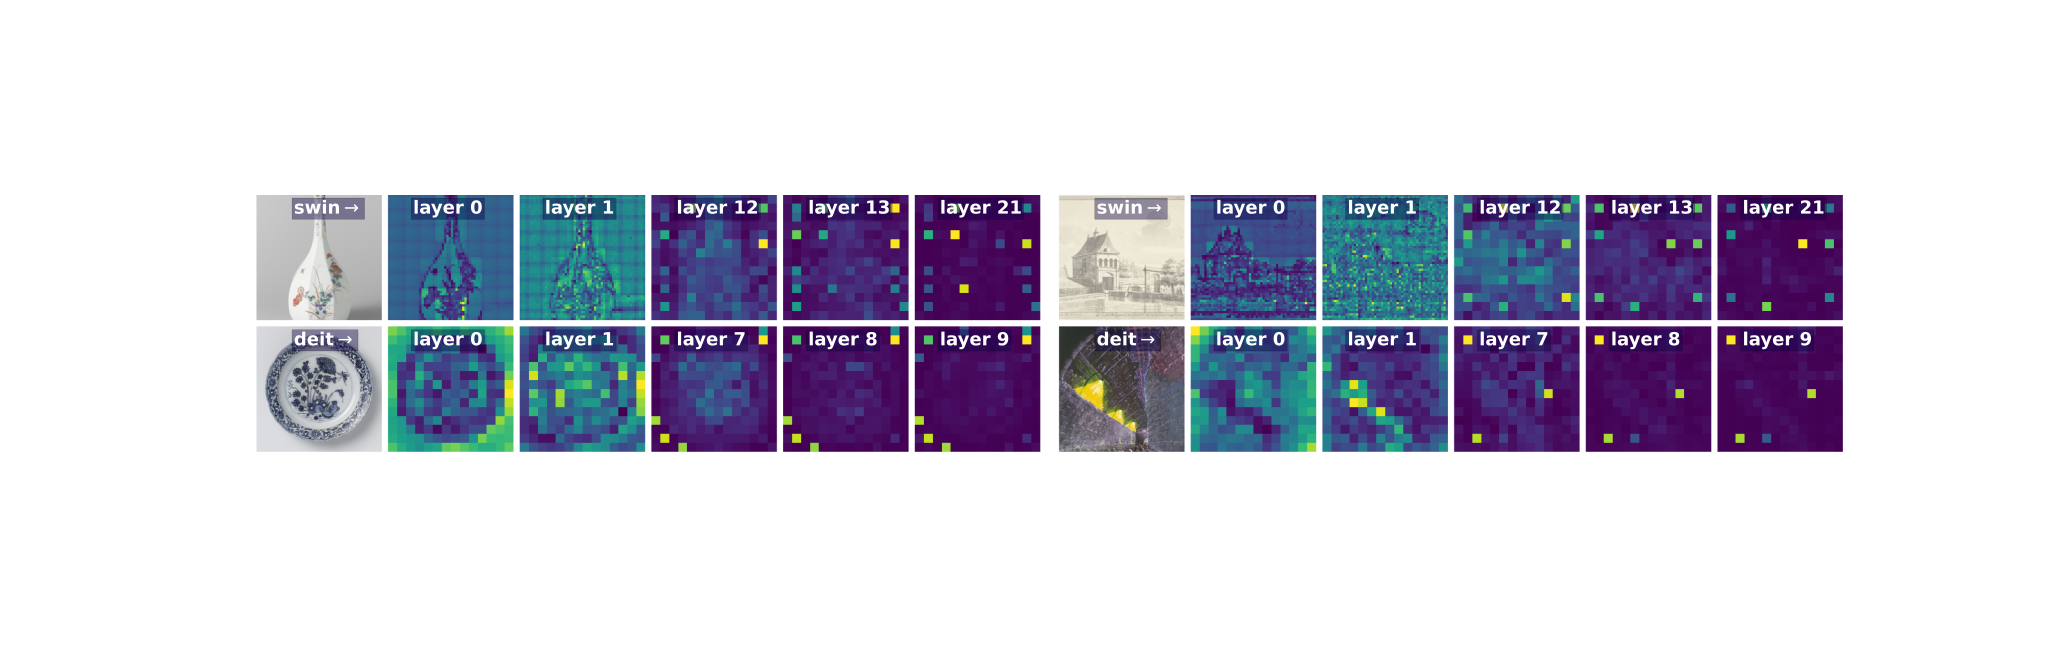
\includegraphics[width=\textwidth]{img/layers.png}
    \caption{Attention layers of successively deeper transformer blocks. One can recognise the input image in earlier layers, while for later ones activation seems sporadic. For \texttt{DeiT}, attention with respect to the class-token is plotted. \texttt{Swin}, on the other hand, does not have a class-token, so average overall attention is used instead. In addition, the window-shifting operations of this architecture are counteracted.}
    \label{results:img:layers}
\end{figure*}

While results are in line with previous studies, it was still surprising to see that VTs showed such good OTS learning performance in section \ref{results:ots}. It suggests that these transformer based architectures are able to give a very complete, high level encoding of the input image. For CNNs this is commonly thought to be true, as they are often described as hierarchical feature extractors that build successively higher level feature maps from lower level ones (see section \ref{intro:cnns}). If the same is true for VTs, is not well understood at this moment. Or at least to the best of the author's knowledge, that is.

A hint of an answer can, however, be found when plotting activation of successively deeper attention layers, as is done in figure \ref{results:img:layers}. While earlier layers retain much spatial information, later ones show more sporadic activation patters. This is what one might expect from an hierarchical feature extractor: the random pixels lighting up might then, for example, correspond to specific, high level properties of the input. Nevertheless, it should be emphasised that no strong conclusions should be drawn from these images, and that more research is required to understand how VTs function.
% Also mention that this was unexpected (but in line with blabla);
% Feature extractor/hierarchical representation building
% Layers img.
% Maybe mention that image specific inductive bias isn't a problem for swin? TODO somewhere else!

\subsubsection{Fine-tuning}

\paragraph{How do these results compare to related studies?}
That the \texttt{Swin} VT performs well after FT, is again consistent with \citeauthor{zhou2021convnets} (\citeyear{zhou2021convnets}). That paper, however, also shows \texttt{ViT} outperforming the \texttt{ResNet101} and \texttt{ResNet152} CNNs. This differs from the results in table \ref{results:tab:ft}, where \texttt{ViT} does not perform well overall, and with 90.11\% even shows the worst testing accuracy on \textit{Type classification}. \texttt{ResNet50} achieves 91.78\% here, and testing the same \texttt{ResNet} versions \citeauthor{zhou2021convnets} used, gives 91.96\% ($\pm$ 0.59\%) accuracy for \texttt{ResNet101}, and 91.94\% ($\pm$ 0.25) for \texttt{ResNet152}.

Results are also less favourable for VTs compared to \citeauthor{matsoukas2021time} (\citeyear{matsoukas2021time}). In that paper the `tiny' version of \texttt{DeiT} outperforms \texttt{ResNet50}, while in table \ref{results:tab:ft} this same \texttt{ResNet50} performs slightly better than the `base' version of \texttt{DeiT}. Going `tiny' also does not help: on \textit{Type classificaiton}, for instance, `tiny' \texttt{DeiT} gets 90.44\% ($\pm$ 0.93\%), which is even worse than `base' \texttt{DeiT}'s 91.78\% in table \ref{results:tab:ots}.

These slight performance differences could be attributable to the different datasets used. In that case, it seems, VTs have certain strengths that those other datasets take more advantage of. Alternatively, it could also be that hyperparameters and regularisation could still be improved. The reason for thinking this, is that preliminary experiments suggested that VTs benefit more from regularisation than CNNs do.

Finally, it was observed that \texttt{ResNet50} appears to flourish with FT, sometimes even beating Conv\-Next in the rankings. This is consistent with \citeauthor{sabatelli2018deep} (\citeyear{sabatelli2018deep}), where it was the best FT model overall.

%FT results in this work also seem less favourable for VTs compared to \citeauthor{zhou2021convnets} (\citeyear{zhou2021convnets}). \texttt{ViT} consistently falls behind \texttt{ResNet50}, and even shows the worst accuracy in table \ref{results:tab:ft} (90.11\%), while in \citeauthor{zhou2021convnets} it was \texttt{ViT} that outperformed \texttt{ResNet101} and 152. It should be mentioned that these two alternatives show performance similar to \texttt{ResNet50}, with type classification accuracies of 91.96\% ($\pm$ 0.59\%) and 91.94\% ($\pm$ 0.25), respectively. Lastly, what is consistent with \citeauthor{zhou2021convnets}, is the good performance of \texttt{Swin} mentioned above.

% Maybe better hyperparameters possible?

%\texttt{VGG19} has dropped further in the rankings, and now shows the worst balanced accuracy for type classification. \texttt{ResNet50}, on the other hand, appears to flourish with FT, often even beating Conv\-Next in the rankings. This is consistent with \citeauthor{sabatelli2018deep} (\citeyear{sabatelli2018deep}), where it was the best FT model overall.

\paragraph{Do CNNs gain more from FT than VTs?}
% Show saliency maps here

\subsubsection{Scaling}

\paragraph{What can be concluded from these results?}
% This, then, does not suggest that at some point OTS learning becomes preferred due to overfitting problems for FT.

\paragraph{Are there any shortcomings?}
% Same training/testing/validating split used. Was that smart? Defense: 5 runs so that makes up for too small testing sets

\subsubsection{Overall}

\paragraph{Why does \textit{Artist classification} show the best overall performance?}
% Sabatelli different
% GINI COEFFICIENTS HYPOTHESIS!!!:
% This seems counterintuitive, as one would think artist identification is much more challenging than determining if something is a painting, or if it is made out of paper instead of wood. An explanation can likely be found in table \ref{methods:datasets}, which shows that material and artist classification sets are the least and most balanced, respectively. In addition, tables \ref{results:tab:ots_type} through \ref{results:tab:ots_artist} show that balanced accuracies are up to 14\% lower than plain ones for material classification, while they are much closer for artist classification. This suggests much accuracy is lost by misclassifying instances of less occurring classes in favor of more occurring ones. Similar finding can be done for FT results in section \ref{results:ft}.

\paragraph{The same hyperparameters are used for all models. Is this fair?}
% Preliminary studies
% Not about getting the best overall performance, but seeing how they compare to one another
% Asterix is that VTs might be able to do better, but then again -> Its also about ease of use

\paragraph{To what extent are the chosen models representative for all VTs and CNNs?}

\paragraph{What can be concluded from the results presented?}

